\section{Implementing CustomGraphSearch}
 %\setcounter{page}{2}
 %\addtocounter{section}{1}
 \thispagestyle{empty}
\subsection{Aim}

This second lab session explores the concept of graph search algorithms. The
agent is still a Vacuum cleaner evolving in a simple grid.
Each square of that grid is either clean filled with dirt, or a wall.
The vacuum cleaner uses search algorithm to locate the dirt squares.
The purpose of this lab is to write our own implementation of
\textit{Breadth First Search} and \textit{Depth First Search} algorithms which
inherit from a \textit{CustomGraphSearch} class.

Using the Java GUI included in the project files, it is possible to compare the
efficiency of differents search algorithms : BFS, DFS, IDS, A*.

%\begin{itemize}
%  \item Turning 90° in the given direction (\textit{uMovement equal to 0})
%  \item Moving forward, down to the next grid line (\textit{uMovement equal to 1})
%  \item Turning again in the same direction (\textit{uMovement equal to 0 again})
%\end{itemize}

\subsection{Implementation}

Given that the course book and the slides provide us with pseudo code of those
algorithms, \textit{figures 3.7 and 3.11}, it is almost only necessary to translate it in Java.

The CustomDepthFirstSearch and CustomBreadthFirstSearch both inherit from
CustomGraphSearch. In terms of pseudo code the only difference between
them is the handling of the \textit{frontier}. Indeed this collection is a
\textit{LIFO} in DFS while a \textit{FIFO} in BFS. The skeleton provide us with
a very simple way of dealing with this issue. Thanks to the boolean \textit{insertFront},
it is possible to add nodes in the front or in the back of the queue depending
on the algorithm, and therefore simulate a LIFO and FIFO.

Thus, to create a CustomBreadthFirstSearch object, the constructor just call the
superclass with \textit{insertFront} being false :
\begin{verbatim}
   super(false); // The BFS uses a fifo, insertFront is false
\end{verbatim}

In the main loop while expanding the currentNode, this boolean is tested before
adding the resulting nodes to the frontier.

Each turn the choosen node is tested, if its state match the goalState, the
full path is returned. If the frontier is empty an empty path is returned, the
algorithm failed. Please refer to the code and comments for more details.

The \textit{Figure 1} presents the result of the two implementations compared
to the built-in DFS and BFS algorithms. The results are almost similar in terms of
time and space complexity.

\begin{figure}[h]
    \centering
    \begin{tabular}{cc}
      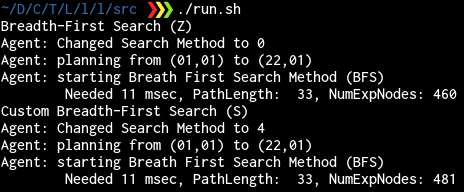
\includegraphics[width=.46\linewidth,scale=1]{./images/lab2_bfs.png} & 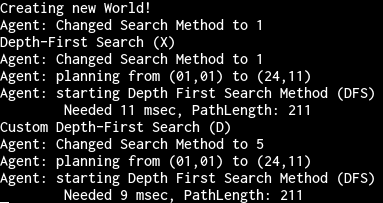
\includegraphics[width=.36\linewidth, scale=1.5]{./images/lab2_dfs.png} \\
      \hspace{0.5cm} (a) & \hspace{0.5cm} (b)
    \end{tabular}
    \caption{Comparison between built-in and custom implementation (a) BFS - (b) DFS \label{fig:BFS and DFS}}
\end{figure}

%\begin{figure}[h]
%    \centering
    %  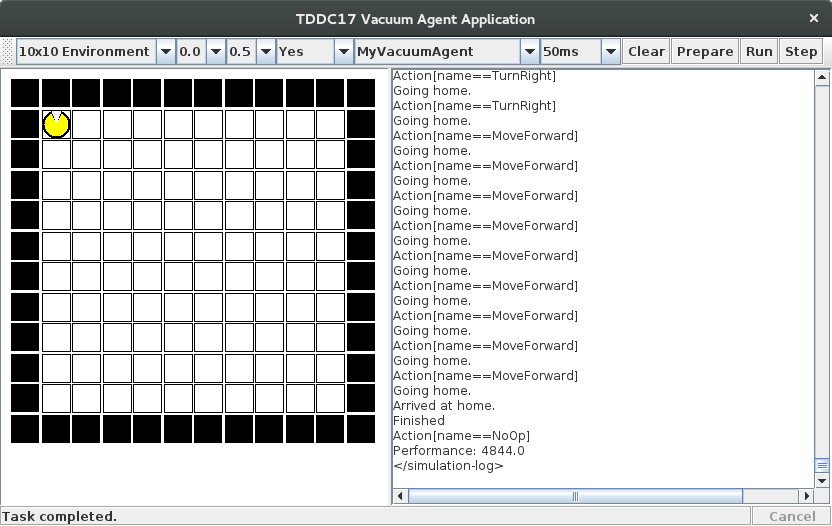
\includegraphics[width=0.83\linewidth]{./images/lab_1.png}
  %  \caption{Screenshot\label{Vacuum cleaner}}
%\end{figure}

\newpage
\thispagestyle{empty}
\section{Theory : questions}

\textit{1. In the vacuum cleaner domain in part 1, what were the states and actions? What is the branching factor?}

In the domain part 1, each square of the grid is a state.
Actions ?
The branching factor \textbf{b} is 8.

\textit{2. What is the difference between Breadth First Search and Uniform Cost Search in a domain where the cost of each action is 1?}

In a domain where the cost of each action is 1, there is no difference between
BFS and Uniform Cost search because every priority is equal to 1.

\textit{3. Suppose that h1 and h2 are admissible heuristics (used in for example A*). Which of the following are also admissible?}

An admissible heuristic never over estimate the cost to reach the goal from n.
Given that h1(n) and h2(n) are admissible, \textbf{(h1+h2)/2} and \textbf{max (h1,h2)}
are also admissible.

\textit{4. If one would use A* to search for a path to one specific square in the vacuum domain, what could the heuristic (h) be? The cost function (g)? Is it an admissible heuristic?}



\textit{5. Draw and explain. Choose your three favorite search algorithms and apply them to any problem domain (it might be a good idea to use a domain where you can identify a good heuristic function). Draw the search tree for them, and explain how they proceed in the searching. Also include the memory usage. You can attach a hand-made drawing.}

\textit{6. Look at all the offline search algorithms presented in chapter 3 plus A* search. Are they complete? Are they optimal? Explain why!}

\textit{7. Assume that you had to go back and do lab 1 once more, but this time with obstacles. Remember that the agent did not have perfect knowledge of the environment but had to explore it incrementally. Could you still use the search algorithms you have learned to guide the agent's execution? What would you search for? Give an example.}
